%!TEX root = ../thesis.tex
\section{強度確認}
設計したロボットアームの強度確認のため,Autodesk Inventorの機能である構造解析を行った.解析における安全率が1以上であれば,強度が十分であると判断した.図\ref{fig:shoulder}に肩部の構成を示す.肩部は,ヨー軸モータとピッチ軸モータを繋ぐ図\ref{fig:shoulder}の部品1,およびリンクの一部である,部品2から構成されている.部品1および部品2には,いずれもアルミニウム合金(A5052)を使用している.

本節では,構造解析による部品の強度確認について述べる.

\begin{figure}[h]
  \centering
  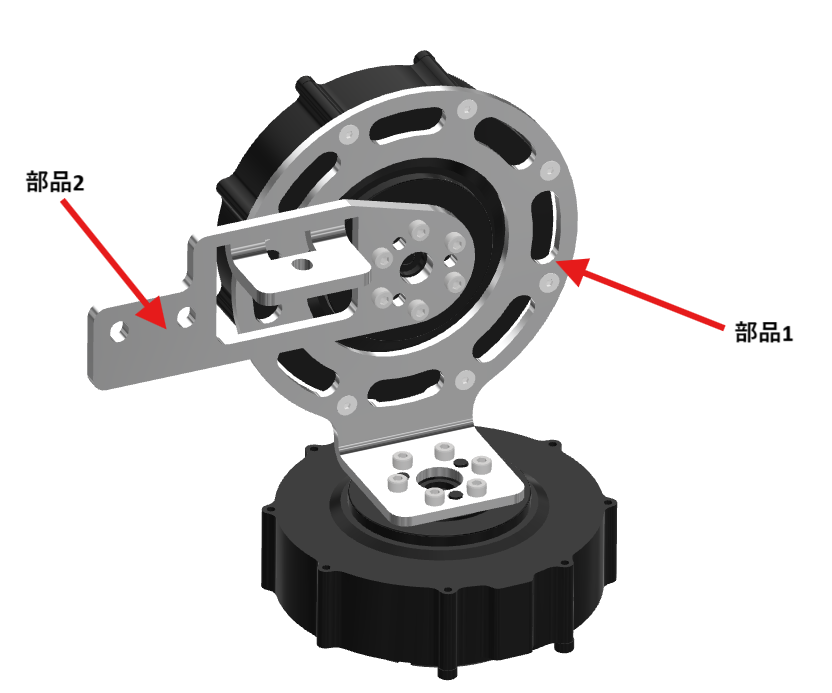
\includegraphics[width=10cm]{images/design/shoulder.png}
  \caption{Configuration of the shoulder components}
  \label{fig:shoulder}
\end{figure}

\subsection{部品1の構造解析}
図\ref{fig:shoulder}の部品1は,ヨー軸モータが最大出力22Nmを発生した際に最大負荷を受ける部品である.図\ref{fig:T3_40}に構造解析結果を示し,設計仕様を表\ref{tab:part1_spec}にまとめた.解析の結果,安全率は0.39であり,強度が不足していることが確認された.特に,図\ref{fig:T3_40}の結果から,曲げ加工部分において強度が不足していることが明らかとなった.この課題を解決するため,「板厚を変更した部品」と「形状を変更した部品」の2つの設計案を検討し,それぞれ再解析を実施した.

\begin{figure}[h]
  \centering
  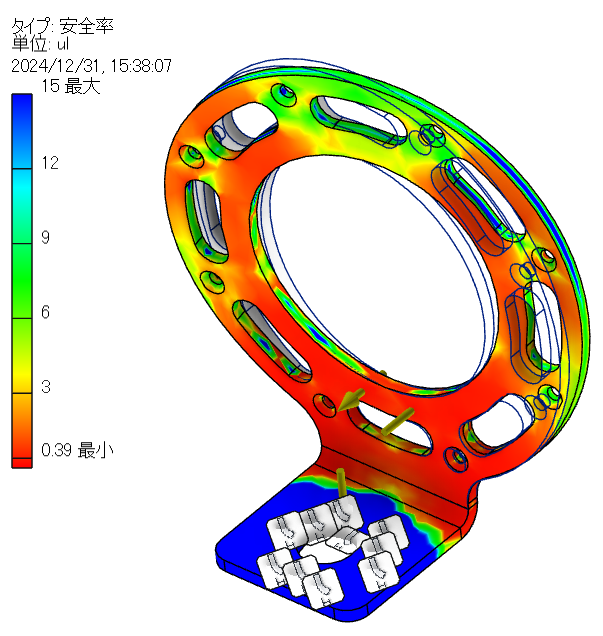
\includegraphics[width=6cm]{images/design/T3_40.png}
  \caption{Structural analysis results of Part 1}
  \label{fig:T3_40}
\end{figure}

\begin{table}[h]
  \centering
  \caption{Specifications of Part 1}
  \begin{tabular}{lc}
    \hline
    厚み & 3㎜ \\ 
    質量 & 43.6g \\ 
    安全率 & 0.39 \\ \hline
  \end{tabular}
  \label{tab:part1_spec}
\end{table}
\clearpage

\subsection{設計の変更}
部品の形状はそのままに,板厚を3mmから5mmに変更した場合の構造解析結果を図\ref{fig:T5}に示し,設計仕様を表\ref{tab:part1_spec_T5}にまとめた.解析の結果,安全率は基準の1を超え,強度が十分であることが確認された.ただし,質量が27.5g増加するという結果が得られた.

\begin{figure}[h]
  \centering
  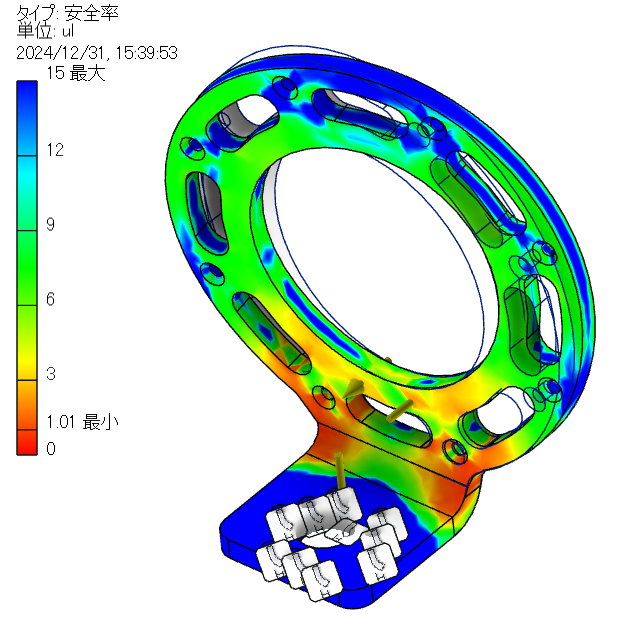
\includegraphics[width=6cm]{images/design/T5.png}
  \caption{Structural analysis results of Part 1 (thickness changed to 5mm)}
  \label{fig:T5}
\end{figure}

\begin{table}[h]
  \centering
  \caption{Specifications of Part 1 (thickness changed to 5mm)}
  \begin{tabular}{lc}
    \hline
    厚み & 5㎜ \\ 
    質量 & 71.1g \\ 
    安全率 & 1.01 \\ \hline
  \end{tabular}
  \label{tab:part1_spec_T5}
\end{table}
\clearpage

次に,板厚を変更せず,形状の改良を行った場合の解析結果を図\ref{fig:T3_80}に示し,設計仕様を表\ref{tab:part1_spec_T3_80}にまとめた.具体的には,図\ref{fig:T3_40}の解析結果を基に,特に強度が不足していると判明した曲げ加工部分の幅を広げる設計変更を行った.

解析の結果,安全率が基準を満たし,十分な強度を確保できることが確認された.また,重量は61.8gであり,板厚を変更した場合(表\ref{tab:part1_spec_T5}参照)と比較して軽量化を実現した.

以上の解析結果を踏まえ,図\ref{fig:shoulder}の部品1について,曲げ加工部分の幅を広げた設計変更を最終設計として採用した.

\begin{figure}[h]
  \centering
  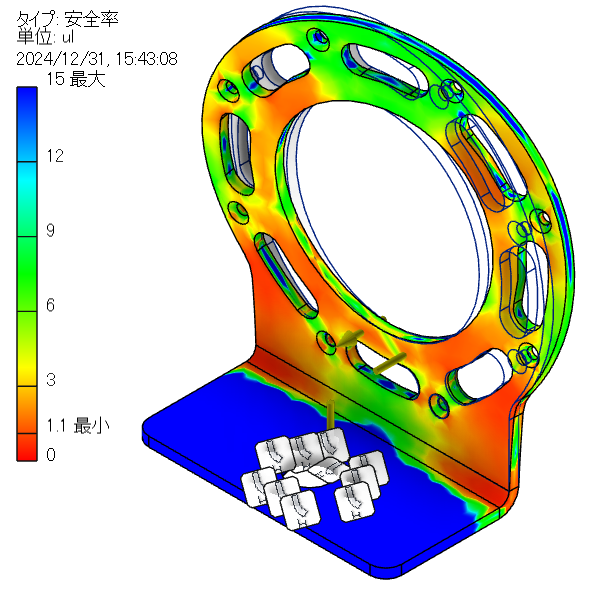
\includegraphics[width=6cm]{images/design/T3_80.png}
  \caption{Structural analysis results of Part 1 (shape optimized)}
  \label{fig:T3_80}
\end{figure}

\begin{table}[h]
  \centering
  \caption{Specifications of Part 1 (shape optimized)}
  \begin{tabular}{lc}
    \hline
    厚み & 3㎜ \\ 
    質量 & 61.8g \\ 
    安全率 & 1.1 \\ \hline
  \end{tabular}
  \label{tab:part1_spec_T3_80}
\end{table}

\subsection{部品2の構造解析}
図\ref{fig:shoulder}の部品2は,アルミフレームを2方向から固定する形状を採用している(図\ref{fig:pitchalumi}参照).最大負荷条件(22Nm)の下で構造解析を実施した結果を図\ref{fig:pitch}に示す.現行の設計では,安全率が0.47と低く,特に赤色で示された箇所において強度不足が確認された.

\begin{figure}[h]
  \centering
  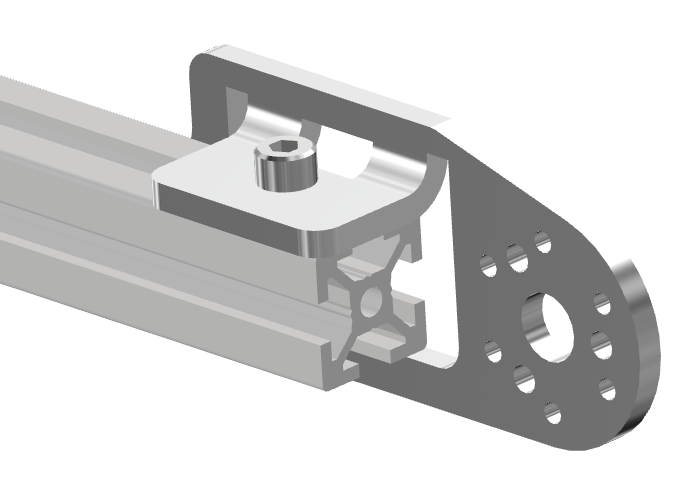
\includegraphics[width=6cm]{images/design/pitchlink.png}
  \caption{Fixing the aluminum frame and part 2}
  \label{fig:pitchalumi}
\end{figure}

\begin{figure}[h]
  \centering
  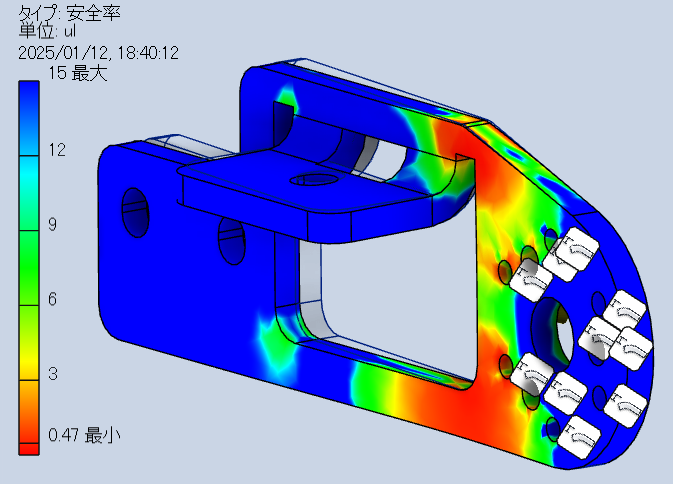
\includegraphics[width=6cm]{images/design/pitch.png}
  \caption{Structural analysis results of Part 2 at maximum output of 22Nm}
  \label{fig:pitch}
\end{figure}

部品の厚みを5mmに変更した場合,安全率は0.58に改善したものの,依然として基準に満たなかった.このため,定格出力(7.5Nm)の条件下で再解析を実施した.解析結果を図\ref{fig:pitchok}に示し,設計仕様を表\ref{tab:part2_spec}にまとめた.この結果,定格条件下では安全率が基準を満たし,十分な強度を確保できることが確認された.

以上より,現設計において部品2の形状変更は行わないこととし,最大出力時の安全率の確保を今後の課題とする.
\begin{figure}[h]
  \centering
  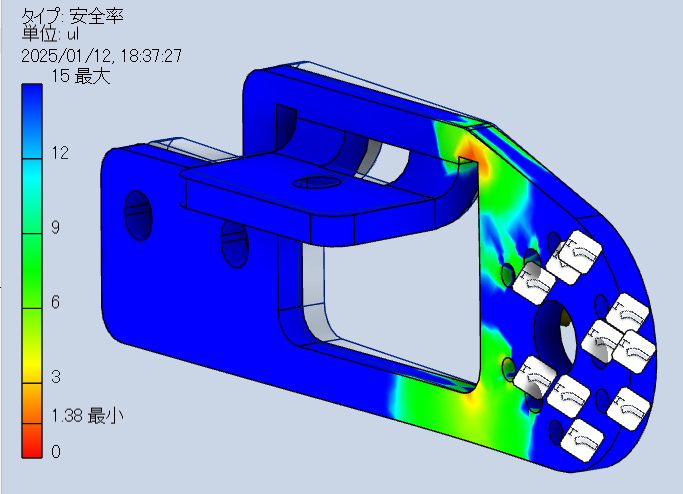
\includegraphics[width=6cm]{images/design/pitchok.png}
  \caption{Structural analysis results of Part 2 at rated output 7.5Nm}
  \label{fig:pitchok}
\end{figure}
\begin{table}[h]
  \centering
  \caption{Specifications of Part 2}
  \begin{tabular}{lc}
    \hline
    厚み & 5㎜ \\ 
    質量 & 34.0g \\ 
    安全率 & 1.38 \\ \hline
  \end{tabular}
  \label{tab:part2_spec}
\end{table}

\newpage